\exercisesetinstructions[\parbox{\linewidth}{A weight of $p$ lb is suspended from a chain of length $\ell$ while a constant force of $\vec F_w$ pushes the weight to the right, making an angle of $\theta$ with the vertical, as shown in the figure below.\\
\null\hfill
\pdftooltip{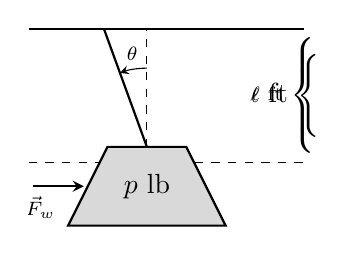
\begin{tikzpicture}
 \draw [dashed] (-1.5,-.2) -- (2,-.2);
 \ifbool{latexml}{
 \draw (1.75,.65) node {$\scriptstyle\ell\textrm{ ft }\Biggl\{$};
 }{
 \draw (1.75,.65) node {\scriptsize $\ell$\ ft $\left\{\rule{0pt}{.8cm}\right.$};
 }
 \filldraw[thick,black,fill=gray!30] (-.5,0) -- (.5,0) -- (1,-1) -- (-1,-1)--cycle;
 \draw (0,-.5) node {$p$ lb};
 \draw [thick] (-1.5,1.5) -- (2,1.5);
 \clip (-1.5,1.5) rectangle (2,-1.25);
 \draw [thick,rotate=110] (0,0) -- (3,0);
 \draw [dashed] (0,0) -- (0,2);
 \draw [rotate=90,->,>=stealth] (1,0) arc (0:20:1);
 \draw [rotate=99] (1.2,0) node {\scriptsize $\theta$};
 \draw [thick,->,>=stealth] (-1.45,-.5) -- (-.8,-.5) node [pos=.15,below] {\scriptsize $\vec F_w$};
\end{tikzpicture}}{ALT-TEXT-TO-BE-DETERMINED}\hfill\null}\\*
In Exercises]{, a force $\vec F_w$ and length $\ell$ are given. Find the angle $\theta$ and the height the weight is lifted as it moves to the right.}

\exercise{$\vec F_w=1$lb, \quad $\ell = 1$ft, \quad $p = 1$lb}{$\theta = 45^\circ$; the weight is lifted $0.29$ ft (about 3.5in).}

\exercise{$\vec F_w=1$lb, \quad $\ell = 1$ft, \quad $p = 10$lb}{$\theta = 5.71^\circ$; the weight is lifted $0.005$ ft (about 1/16th of an inch).}

\exercise{$\vec F_w=1$lb, \quad $\ell = 10$ft, \quad $p = 1$lb}{$\theta = 45^\circ$; the weight is lifted $2.93$ ft.}

\exercise{$\vec F_w=10$lb, \quad $\ell = 10$ft, \quad $p = 1$lb}{$\theta = 84.29^\circ$; the weight is lifted $9$ ft.}

\exercisesetend
